\documentclass[nohyperref]{article}

\usepackage{icml2026_weightsymmetry}
\usepackage{amsmath}
\usepackage{amssymb}
\usepackage{booktabs}
\usepackage{graphicx}
\usepackage{subcaption}
\usepackage{tikz}
\usepackage{xcolor}
\usepackage{microtype}
\usepackage{placeins}

\usetikzlibrary{arrows.meta,positioning,calc}
\setlength{\textfloatsep}{6pt plus 1pt minus 2pt}
\setlength{\floatsep}{6pt plus 1pt minus 2pt}
\setlength{\intextsep}{6pt plus 1pt minus 2pt}

\icmltitlerunning{Low-Rank Networks Recover Weight and Functional Symmetry Better}

\begin{document}
\raggedbottom

\twocolumn[
\icmltitle{Low-Rank Networks Recover Weight and Functional Symmetry Better}

\begin{icmlauthorlist}
\icmlauthor{Anonymous Author(s)}{anon}
\end{icmlauthorlist}
\icmlaffiliation{anon}{Anonymous Institution}
\icmlcorrespondingauthor{Anonymous Author}{anonymous@example.com}
\icmlkeywords{weight-space symmetry, low-rank networks, random features, implicit bias, representation symmetry}

\vskip 0.2in
]

\printAffiliationsAndNotice{}

\begin{abstract}
We study an empirical phenomenon in low-rank random-feature networks: even when stochastic training sees one non-symmetrized sample at a time, the learned model can recover a globally symmetric function and, in successful regimes, symmetric internal partial functions.
The effect is not explained by output invariance alone.
Low-loss counterexamples exist where the output is nearly symmetric but the learned partial functions remain asymmetric.
We therefore analyze symmetry simultaneously in function space, representation space, and weight space.
Across one-dimensional sum of cosines experiments and new multidimensional batch-size-one experiments, low-rank bottleneck networks exhibit a distinctive regime where symmetry is visible in late partial functions and in mirror-paired first-layer atoms with matched outgoing weights.
\end{abstract}

\section{Question}

Weight-space symmetries are usually discussed as exact parameter transformations that preserve a network function, especially in model merging and mode connectivity \citep{garipov2018loss,frankle2020linear,entezari2022role,ainsworth2023git}.
Here we ask a different question: can optimization discover a \emph{data-dependent} symmetry in weight space when the training procedure itself is maximally asymmetric?
Our motivating setting uses a target invariant under $x \mapsto -x$ or related finite transformations, but trains with stochastic batch size one and without paired samples.
The surprising observation is that RF-LR models often learn not only an invariant output but also invariant low-rank partial functions.
Our weight-space test asks whether this functional symmetry is accompanied by an organization of the trained parameters themselves: first-layer atoms should appear in approximate mirror pairs, and the low-rank outgoing coefficients attached to paired atoms should agree.

For a learned scalar function $f$, we measure
\[
D_{\mathrm{out}}(T)
=
\frac{\mathbb{E}_{x}\left[(f(x)-f(Tx))^2\right]}
{\mathbb{E}_{x}\left[f(x)^2\right]+\varepsilon},
\]
and apply the same relative defect to active internal partial functions.
For first-layer ReLU atoms $\sigma(a_j^\top x+b_j)$, we also compare each atom to its nearest mirror $(-a_j,b_j)$ and measure the relative mismatch and correlation of their outgoing low-rank weights.
Small mismatch means that symmetry is not only visible after evaluating the network; it is also encoded as paired atoms in weight space.

\section{Low-Rank Architecture}

\begin{figure}[t]
\centering
\resizebox{0.95\linewidth}{!}{
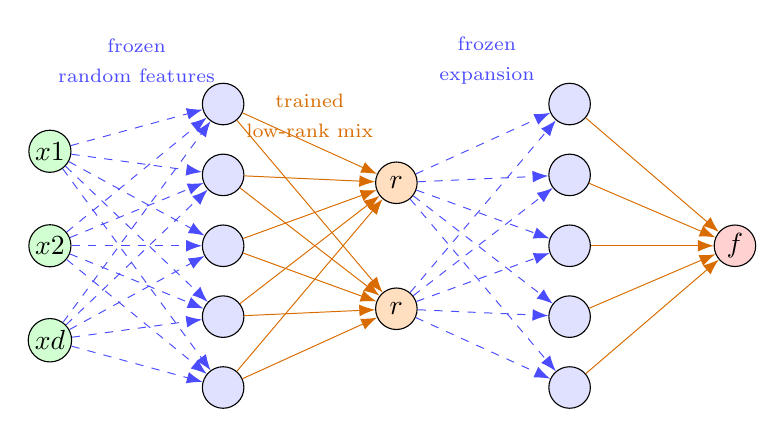
\begin{tikzpicture}[
    layer/.style={circle,draw,minimum size=15pt,inner sep=1pt},
    wide/.style={layer,fill=blue!12},
    rank/.style={layer,fill=orange!25},
    input/.style={layer,fill=green!18},
    output/.style={layer,fill=red!18},
    edge/.style={-{Latex[length=2mm]},line width=0.35pt,black!60},
    frozen/.style={edge,dashed,blue!70},
    trainable/.style={edge,orange!85!black}
]
\foreach \y/\name in {1.2/x1,0/x2,-1.2/xd}
    \node[input] (x\name) at (0,\y) {$\name$};
\foreach \y/\name in {1.8/h1,0.9/h2,0/h3,-0.9/h4,-1.8/h5}
    \node[wide] (h\name) at (2.2,\y) {};
\foreach \y/\name in {0.8/r1,-0.8/r2}
    \node[rank] (r\name) at (4.4,\y) {$r$};
\foreach \y/\name in {1.8/g1,0.9/g2,0/g3,-0.9/g4,-1.8/g5}
    \node[wide] (g\name) at (6.6,\y) {};
\node[output] (out) at (8.7,0) {$f$};
\foreach \x in {xx1,xx2,xxd}
    \foreach \h in {hh1,hh2,hh3,hh4,hh5}
        \draw[frozen] (\x) -- (\h);
\foreach \h in {hh1,hh2,hh3,hh4,hh5}
    \foreach \r in {rr1,rr2}
        \draw[trainable] (\h) -- (\r);
\foreach \r in {rr1,rr2}
    \foreach \g in {gg1,gg2,gg3,gg4,gg5}
        \draw[frozen] (\r) -- (\g);
\foreach \g in {gg1,gg2,gg3,gg4,gg5}
    \draw[trainable] (\g) -- (out);
\node[align=center,blue!70] at (1.1,2.35) {\scriptsize frozen\\[-1pt]\scriptsize random features};
\node[align=center,orange!85!black] at (3.3,1.65) {\scriptsize trained\\[-1pt]\scriptsize low-rank mix};
\node[align=center,blue!70] at (5.55,2.35) {\scriptsize frozen\\[-1pt]\scriptsize expansion};
\end{tikzpicture}}
\caption{RF-LR alternates wide random-feature maps and low-rank bottlenecks. Symmetry is measured at the output, at bottleneck partials, and through mirror structure in first-layer atoms.}
\label{fig:arch}
\end{figure}

We use the finite-width RF-LR model corresponding to the multi-component and multi-layer neural network line of work \citep{zhang2024structured}.
Let $z^{(0)}(x)=x\in\mathbb{R}^{d}$.
For block $\ell=1,\ldots,L$, the network applies
\begin{align*}
u^{(\ell)}(x)
&=
\sigma\!\left(A^{(\ell)} z^{(\ell-1)}(x)+b^{(\ell)}\right),\\
z^{(\ell)}(x)
&=
B^{(\ell)}u^{(\ell)}(x).
\end{align*}
where $A^{(\ell)}\in\mathbb{R}^{W\times r_{\ell-1}}$ and $b^{(\ell)}\in\mathbb{R}^{W}$ are frozen i.i.d.\ random features, while $B^{(\ell)}\in\mathbb{R}^{r_\ell\times W}$ is trained.
The ranks are $r_0=d$, $r_L=1$, and $r_\ell=r\ll W$ for hidden bottlenecks.
Thus each layer first expands to width $W$, then contracts through a trained rank-$r$ channel mixer.
The scalar prediction is $f_\theta(x)=z^{(L)}(x)$.
Equivalently, $A^{(1)}$ is the frozen first feature map, and the entries of $B^{(\ell)}$ are the trainable channel weights.

The internal partial functions are the bottleneck coordinates
\[
p_k^{(\ell)}(x)=z_k^{(\ell)}(x),
\qquad
k=1,\ldots,r_\ell.
\]
These are the objects on which we measure active partial symmetry defects.
The first-layer atom associated with row $a_j$ and bias $b_j$ is $\sigma(a_j^\top x+b_j)$; weight-space symmetry is probed by looking for mirror atoms $\sigma((-a_j)^\top x+b_j)$ and comparing their trained outgoing coefficients in $B^{(1)}$.

The architectural bias is not an explicit equivariance constraint.
The first random-feature layer is sampled asymmetrically, and mini-batches contain a single point.
Nevertheless, the trained low-rank channel weights can organize mirror-related atoms into an approximately symmetric representation.

% Auto-generated by build_paper_assets.py
\vspace{0.2em}
\begin{center}\small
\setlength{\tabcolsep}{4pt}
\renewcommand{\arraystretch}{1.18}
\captionof{table}{Main experimental protocol. Multidimensional data are unpaired: no $(x,-x)$ sample is inserted.}
\label{tab:method-summary}
\begin{tabular}{@{}p{0.27\linewidth}p{0.66\linewidth}@{}}\toprule
Component & Setting \\\midrule
Targets & sum of cosines; Gaussian, quadratic, and soft-axis sign-flip targets \\
\textbf{RF-LR main} & \textbf{$W=512$, $r=8,16$; freeze $A^{(\ell)},b^{(\ell)}$; train only $B^{(\ell)}$} \\
Controls & RF-LR $r=64,128$ and matched MLP checks \\
Training & Adam $10^{-3}$, $10k$ epochs, batch $1$, MSE objective \\
Selection & best held-out MSE checkpoint, then post-hoc symmetry metrics \\
Metrics & test MSE, $D_{out}$, active $D_p$, mirror mismatch \\
\bottomrule\end{tabular}
\end{center}



\section{Evidence}

\paragraph{One-dimensional sum of cosines.}
We train low-loss even sum of cosines configurations with width $1024$ and adaptive SGD.
The target family is $g_m(x)=\sum_{q=1}^{m}\alpha_q\cos(\omega_q x)$ with fixed frequencies and coefficients, following the high-frequency motivation of MMNN/FMMNN models \citep{zhang2024structured,zhang2025fourier}; every term is invariant under $x\mapsto -x$, but training samples are not duplicated with mirrored partners.
This makes the task a controlled probe of whether RF-LR discovers even symmetry from optimization rather than explicit augmentation.
Across six reliable low-loss runs, final test MSE ranges from $1.94\cdot10^{-5}$ to $3.26\cdot10^{-3}$.
Output even defects range from $4.1\cdot10^{-6}$ to $8.0\cdot10^{-4}$, while active last-layer partial even defects range from $6.24\cdot10^{-5}$ to $5.22\cdot10^{-4}$.
This is the cleanest evidence that the learned symmetry is internal, not only an output coincidence.

\begin{figure}[!t]
\centering
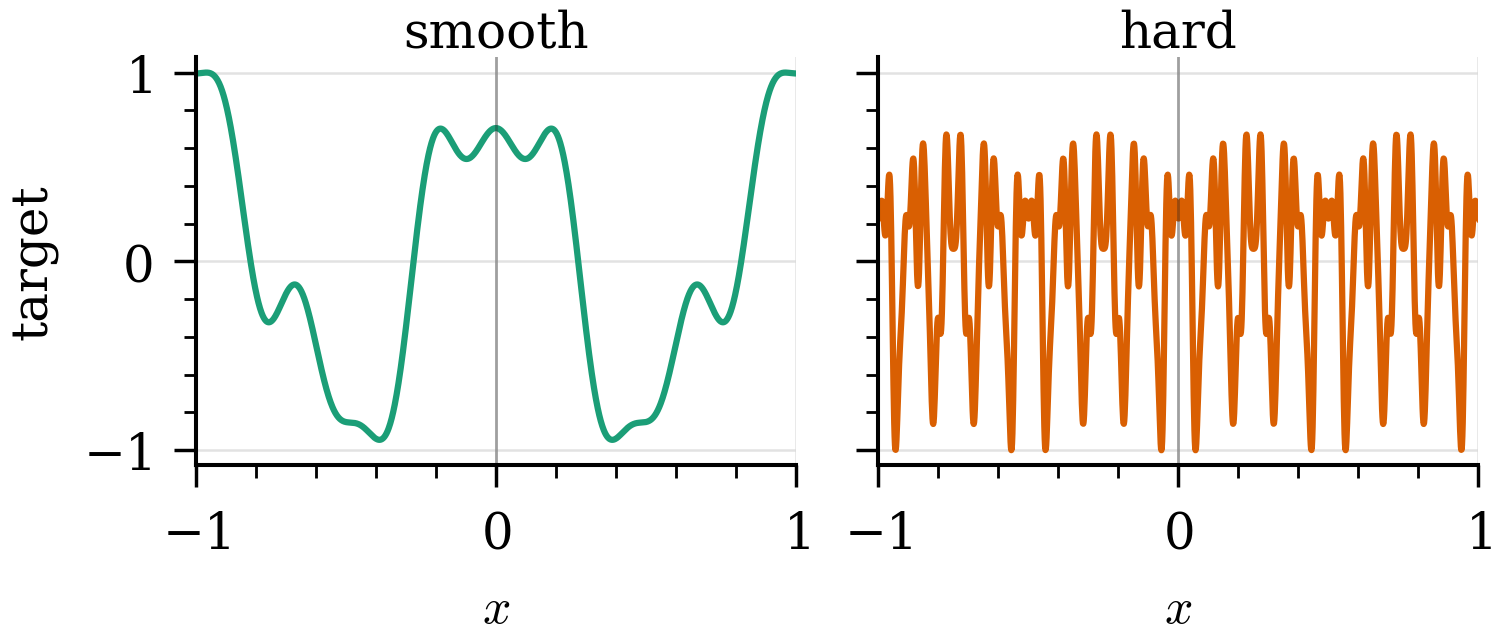
\includegraphics[width=0.98\linewidth]{results/paper_assets/paper_sumcos_targets.png}
\caption{Two one-dimensional sum of cosines targets used as controlled even functions. The smooth target tests low-frequency symmetry recovery; the hard target stresses high-frequency fitting while preserving the same $x\mapsto -x$ symmetry.}
\label{fig:sumcos-targets}
\end{figure}

\begin{figure*}[!t]
\centering
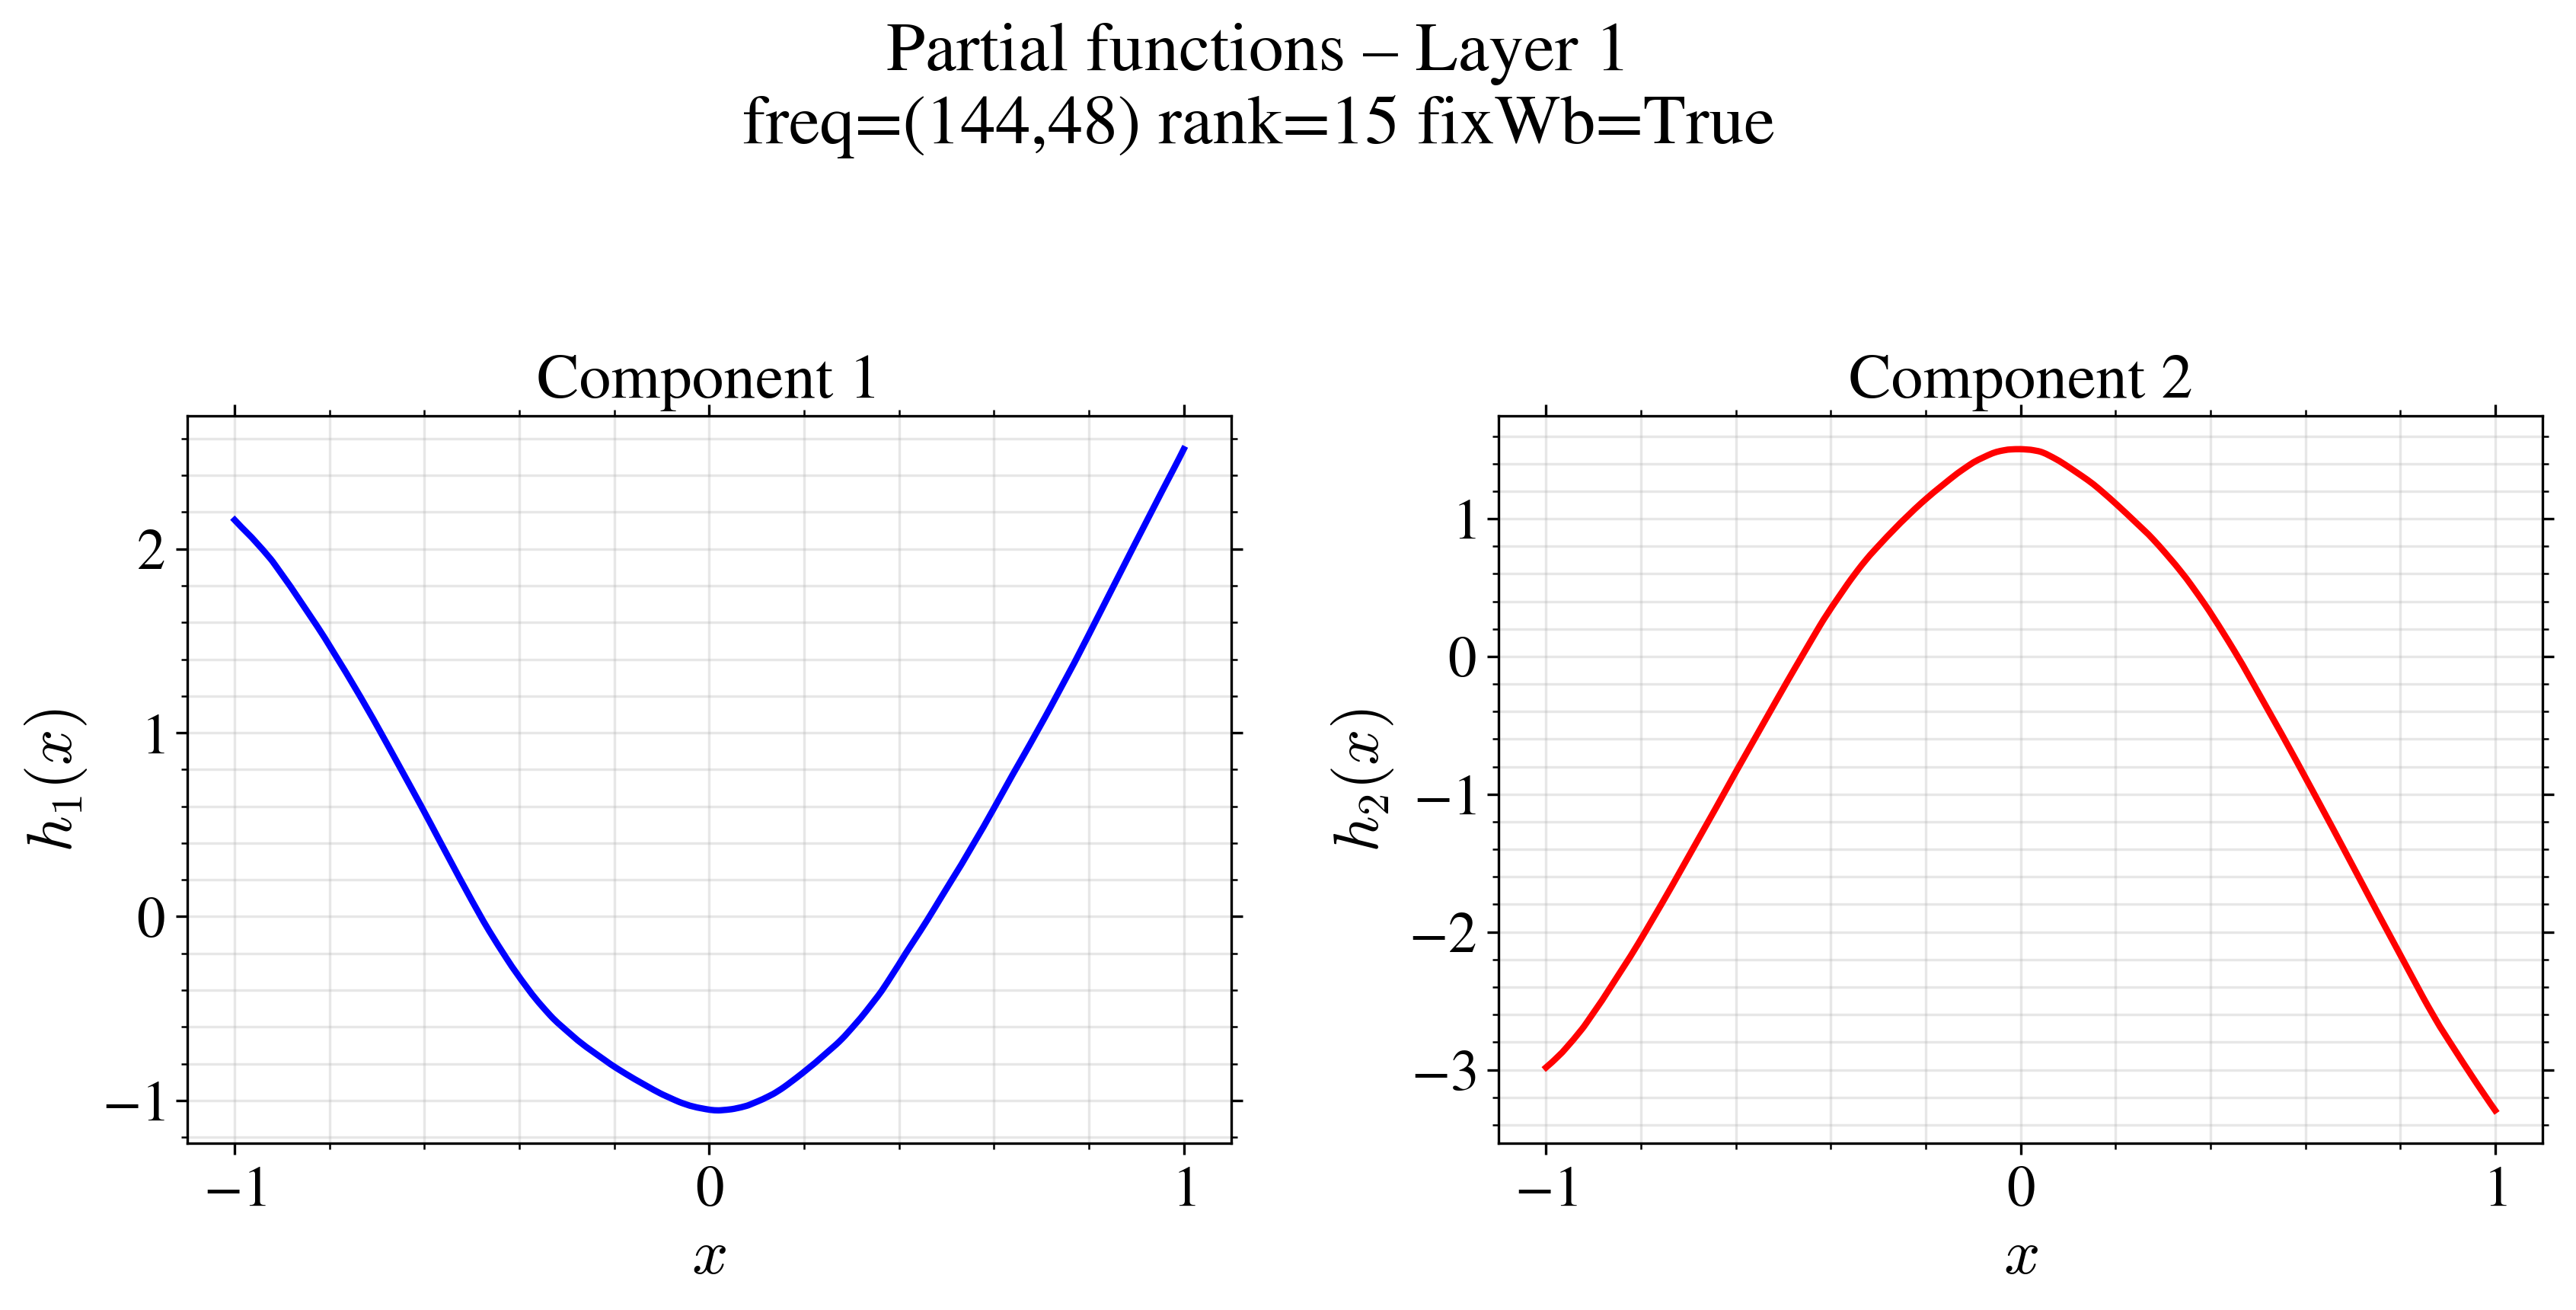
\includegraphics[width=0.47\textwidth]{../icml_sgdadamlandscapedynamical/figures/channel_partials_layer1.png}\hfill
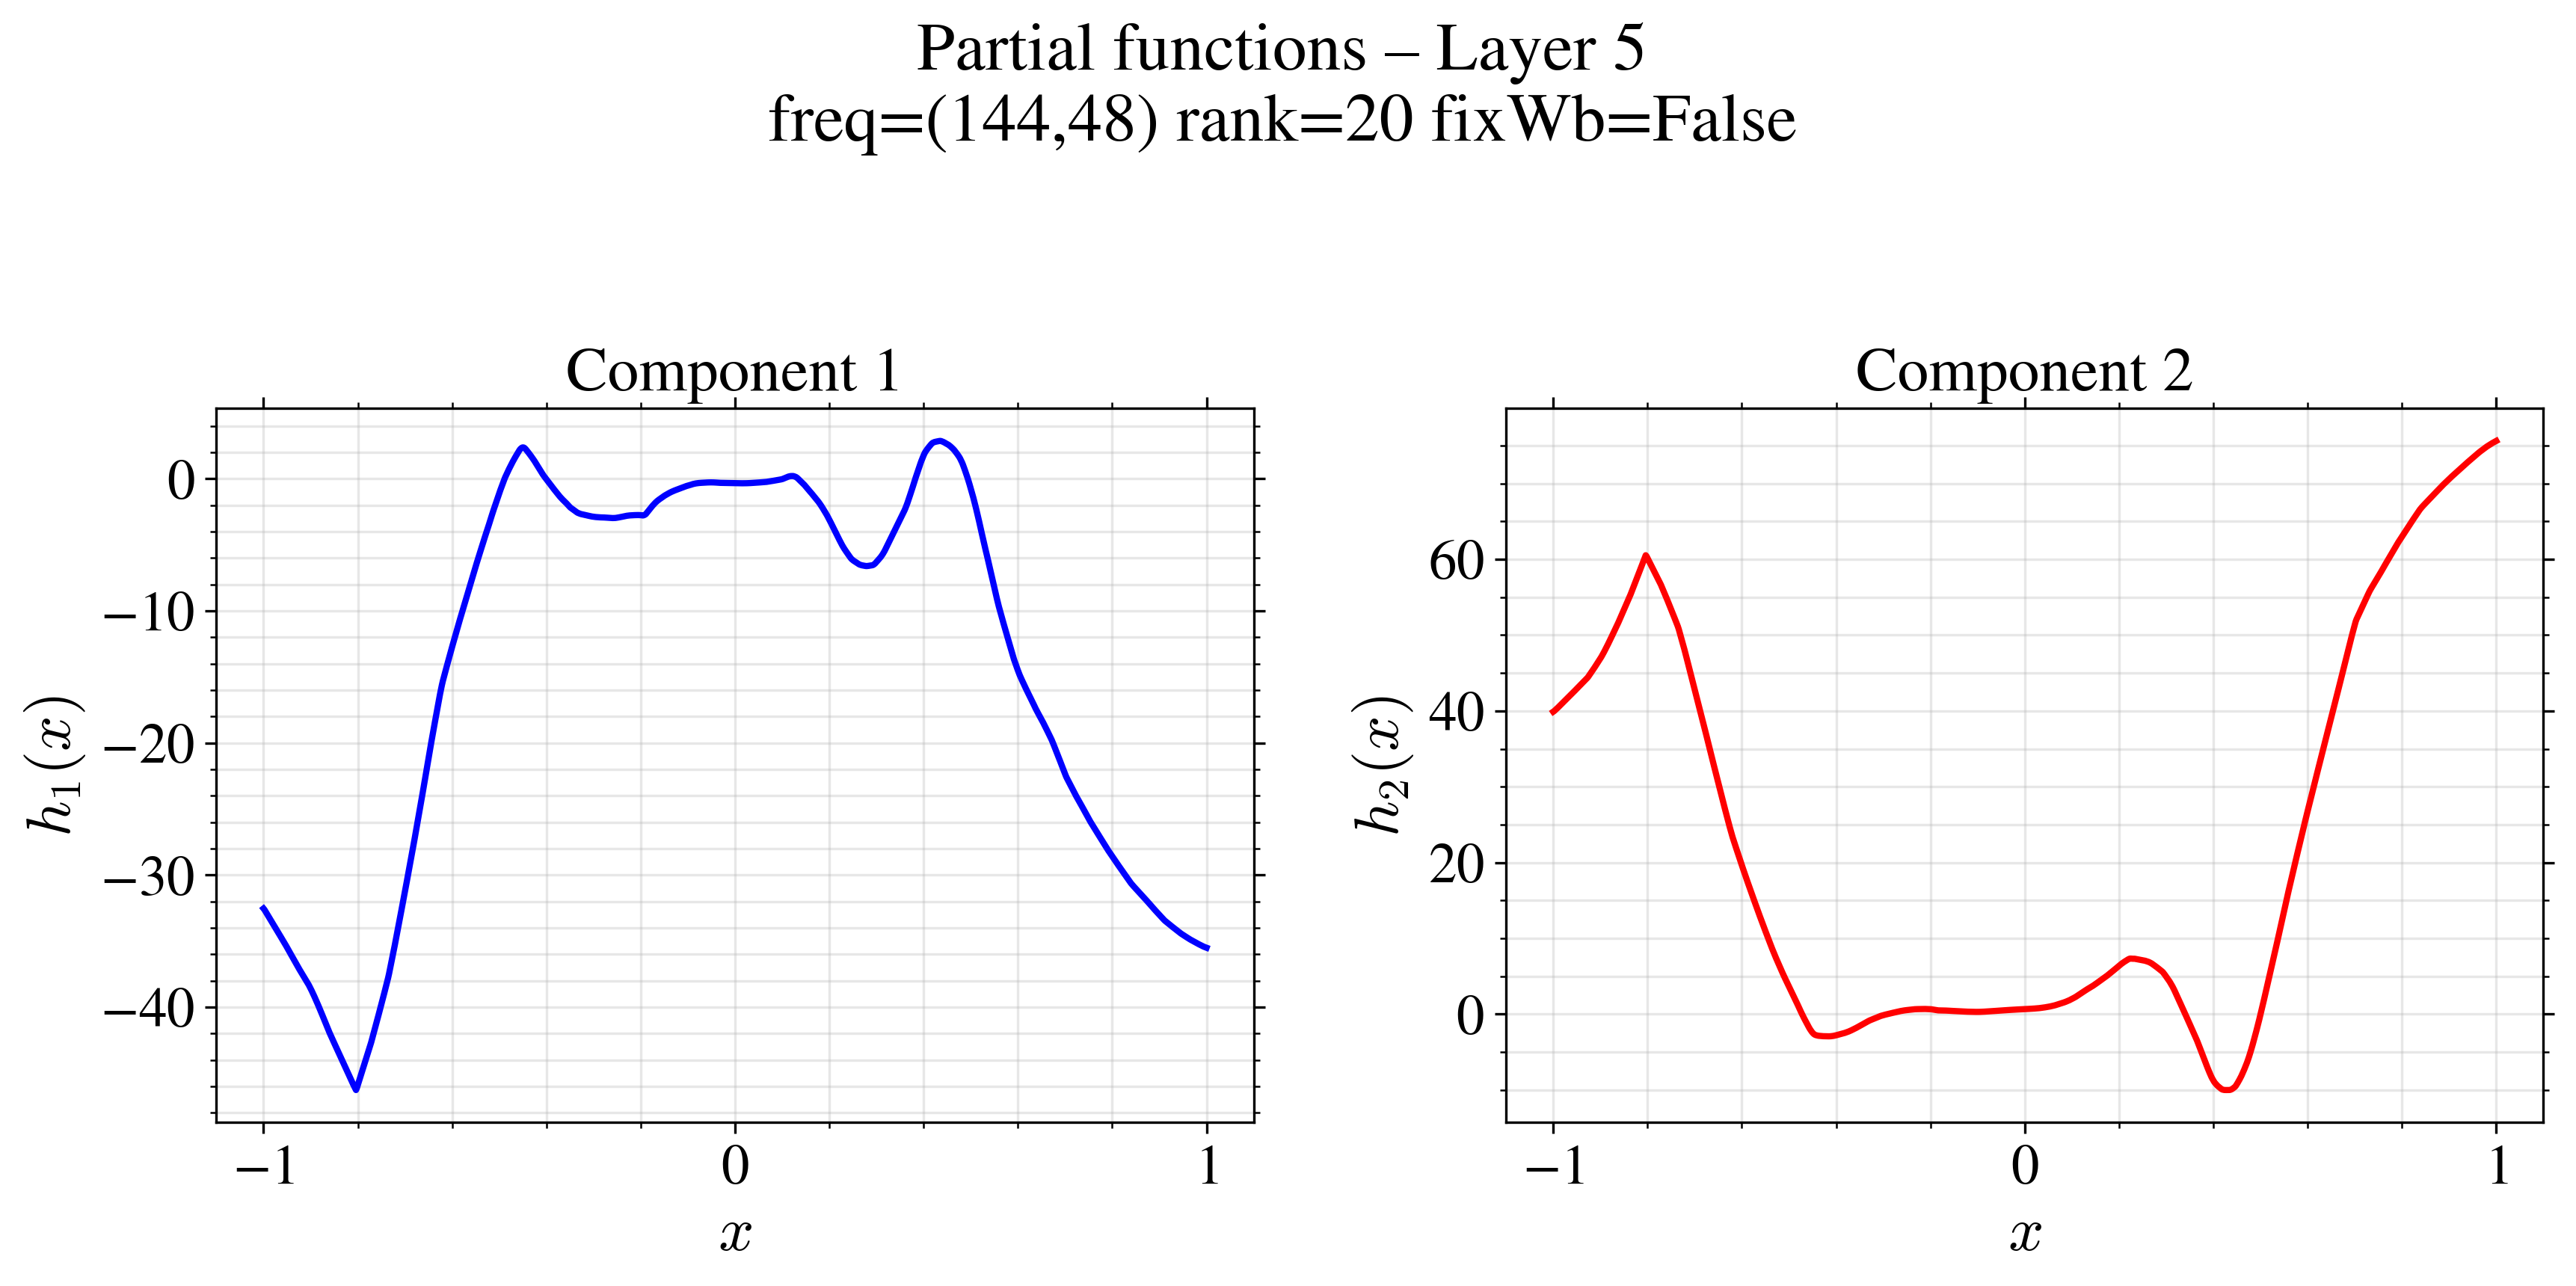
\includegraphics[width=0.47\textwidth]{results/paper_assets/paper_mlp_asymmetry_layer7.png}
\vspace{0.25em}

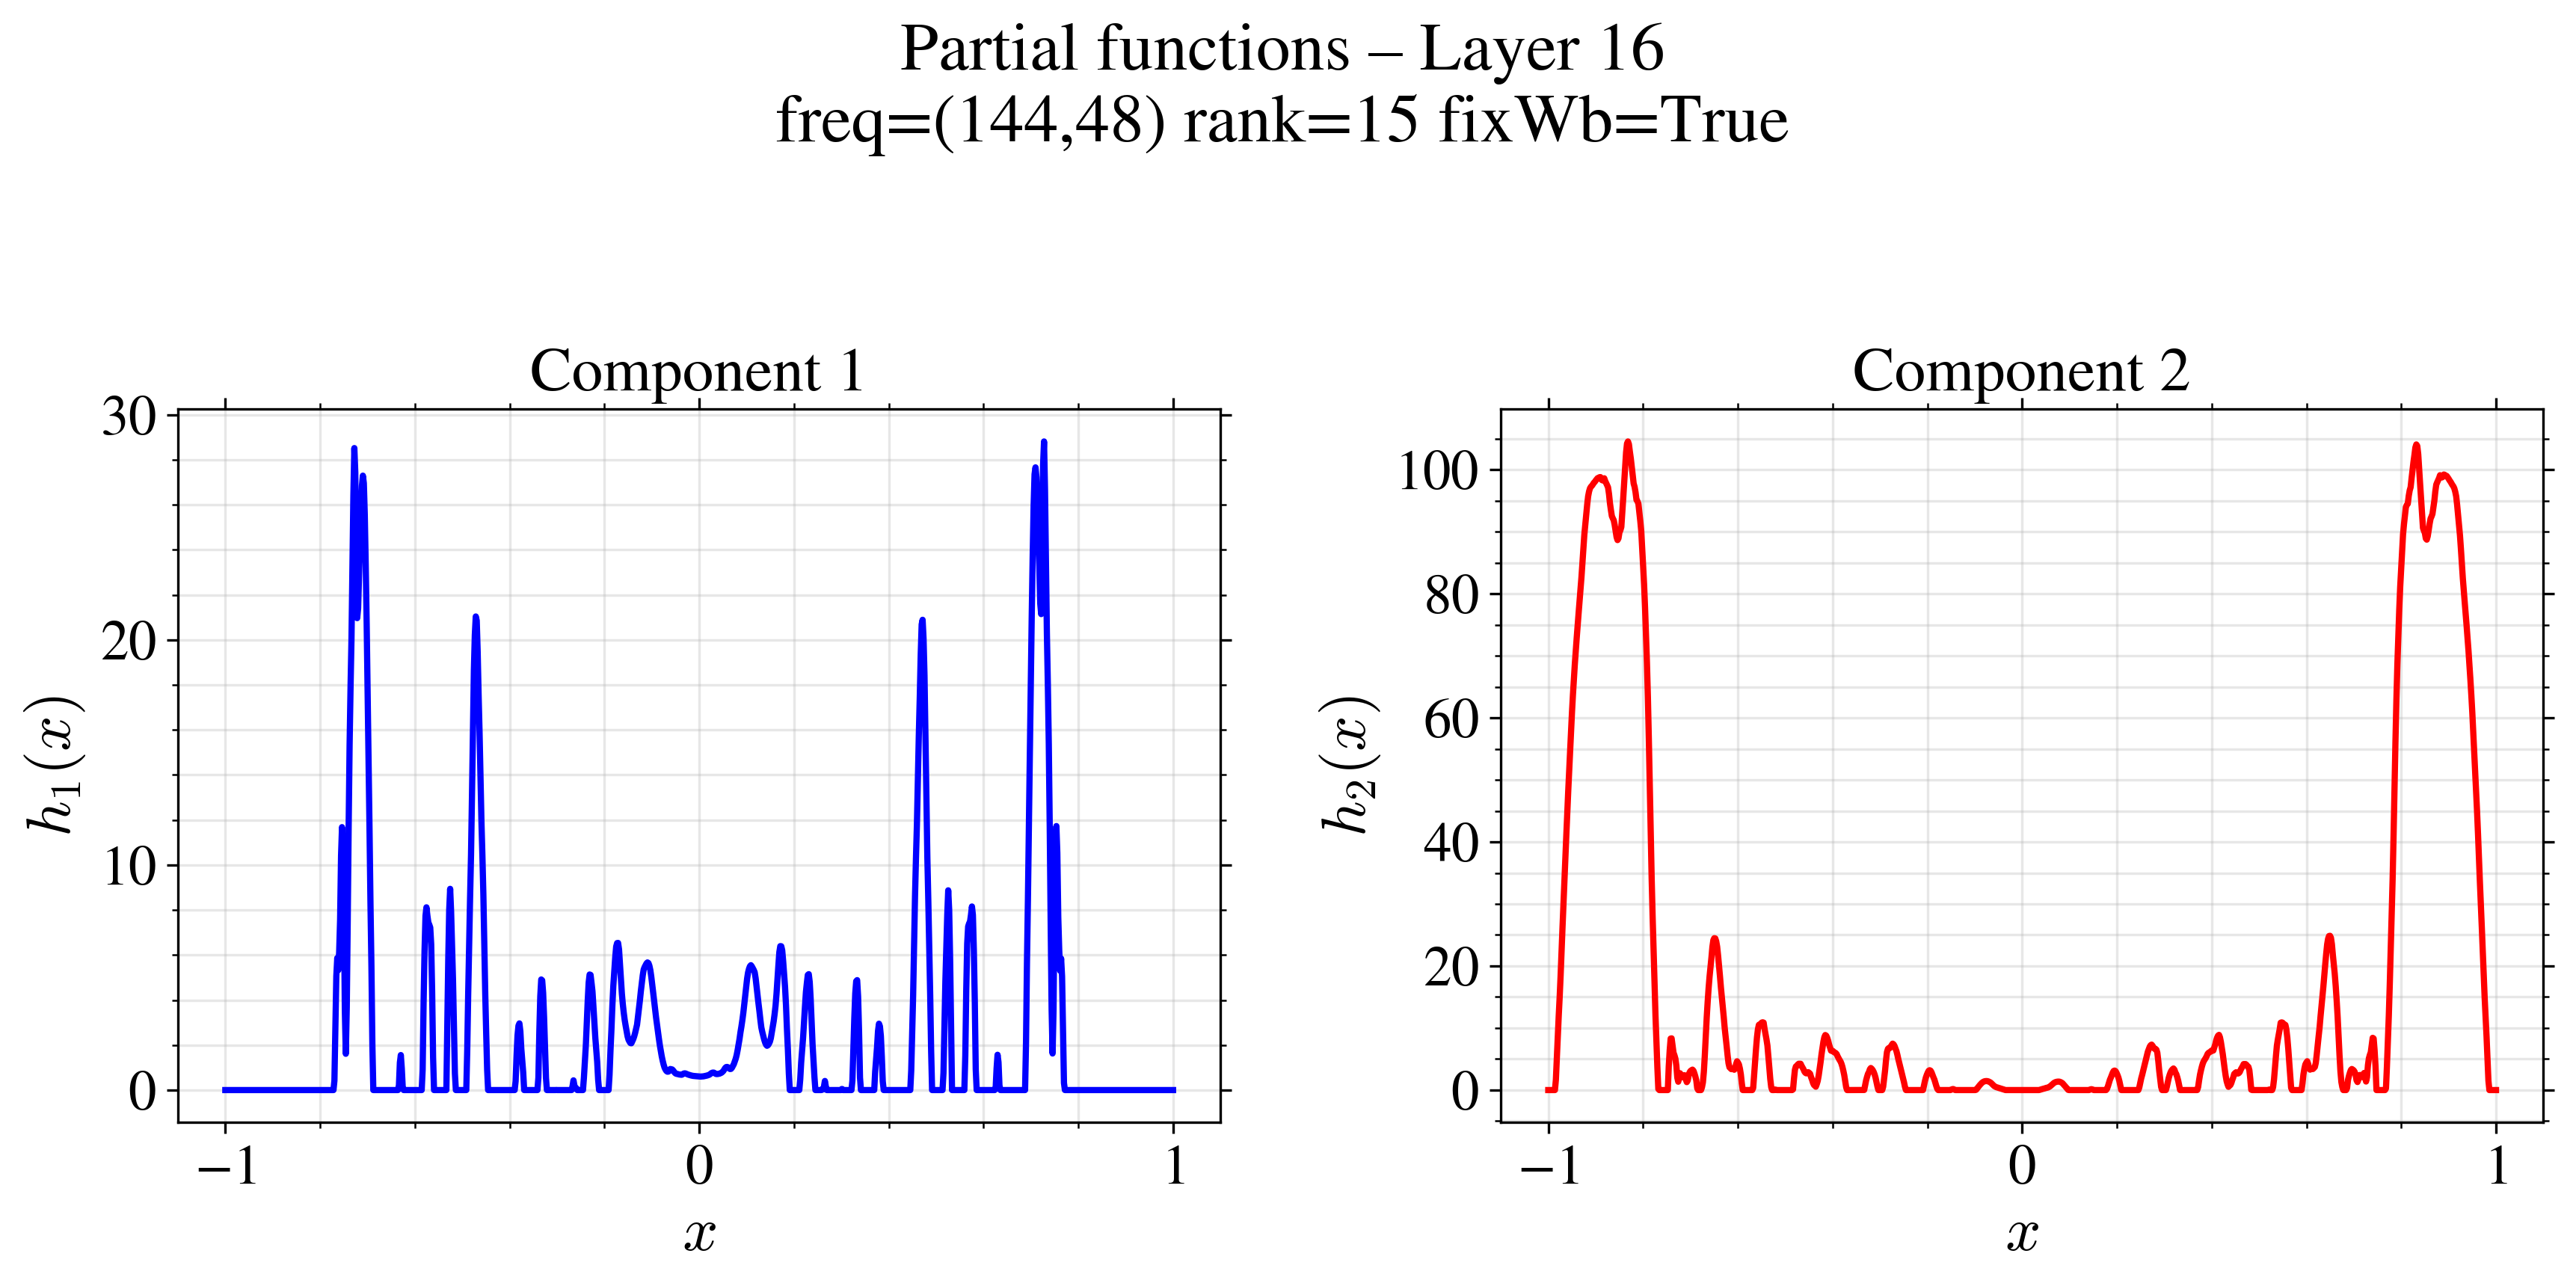
\includegraphics[width=0.47\textwidth]{../icml_sgdadamlandscapedynamical/figures/channel_partials_layer16.png}\hfill
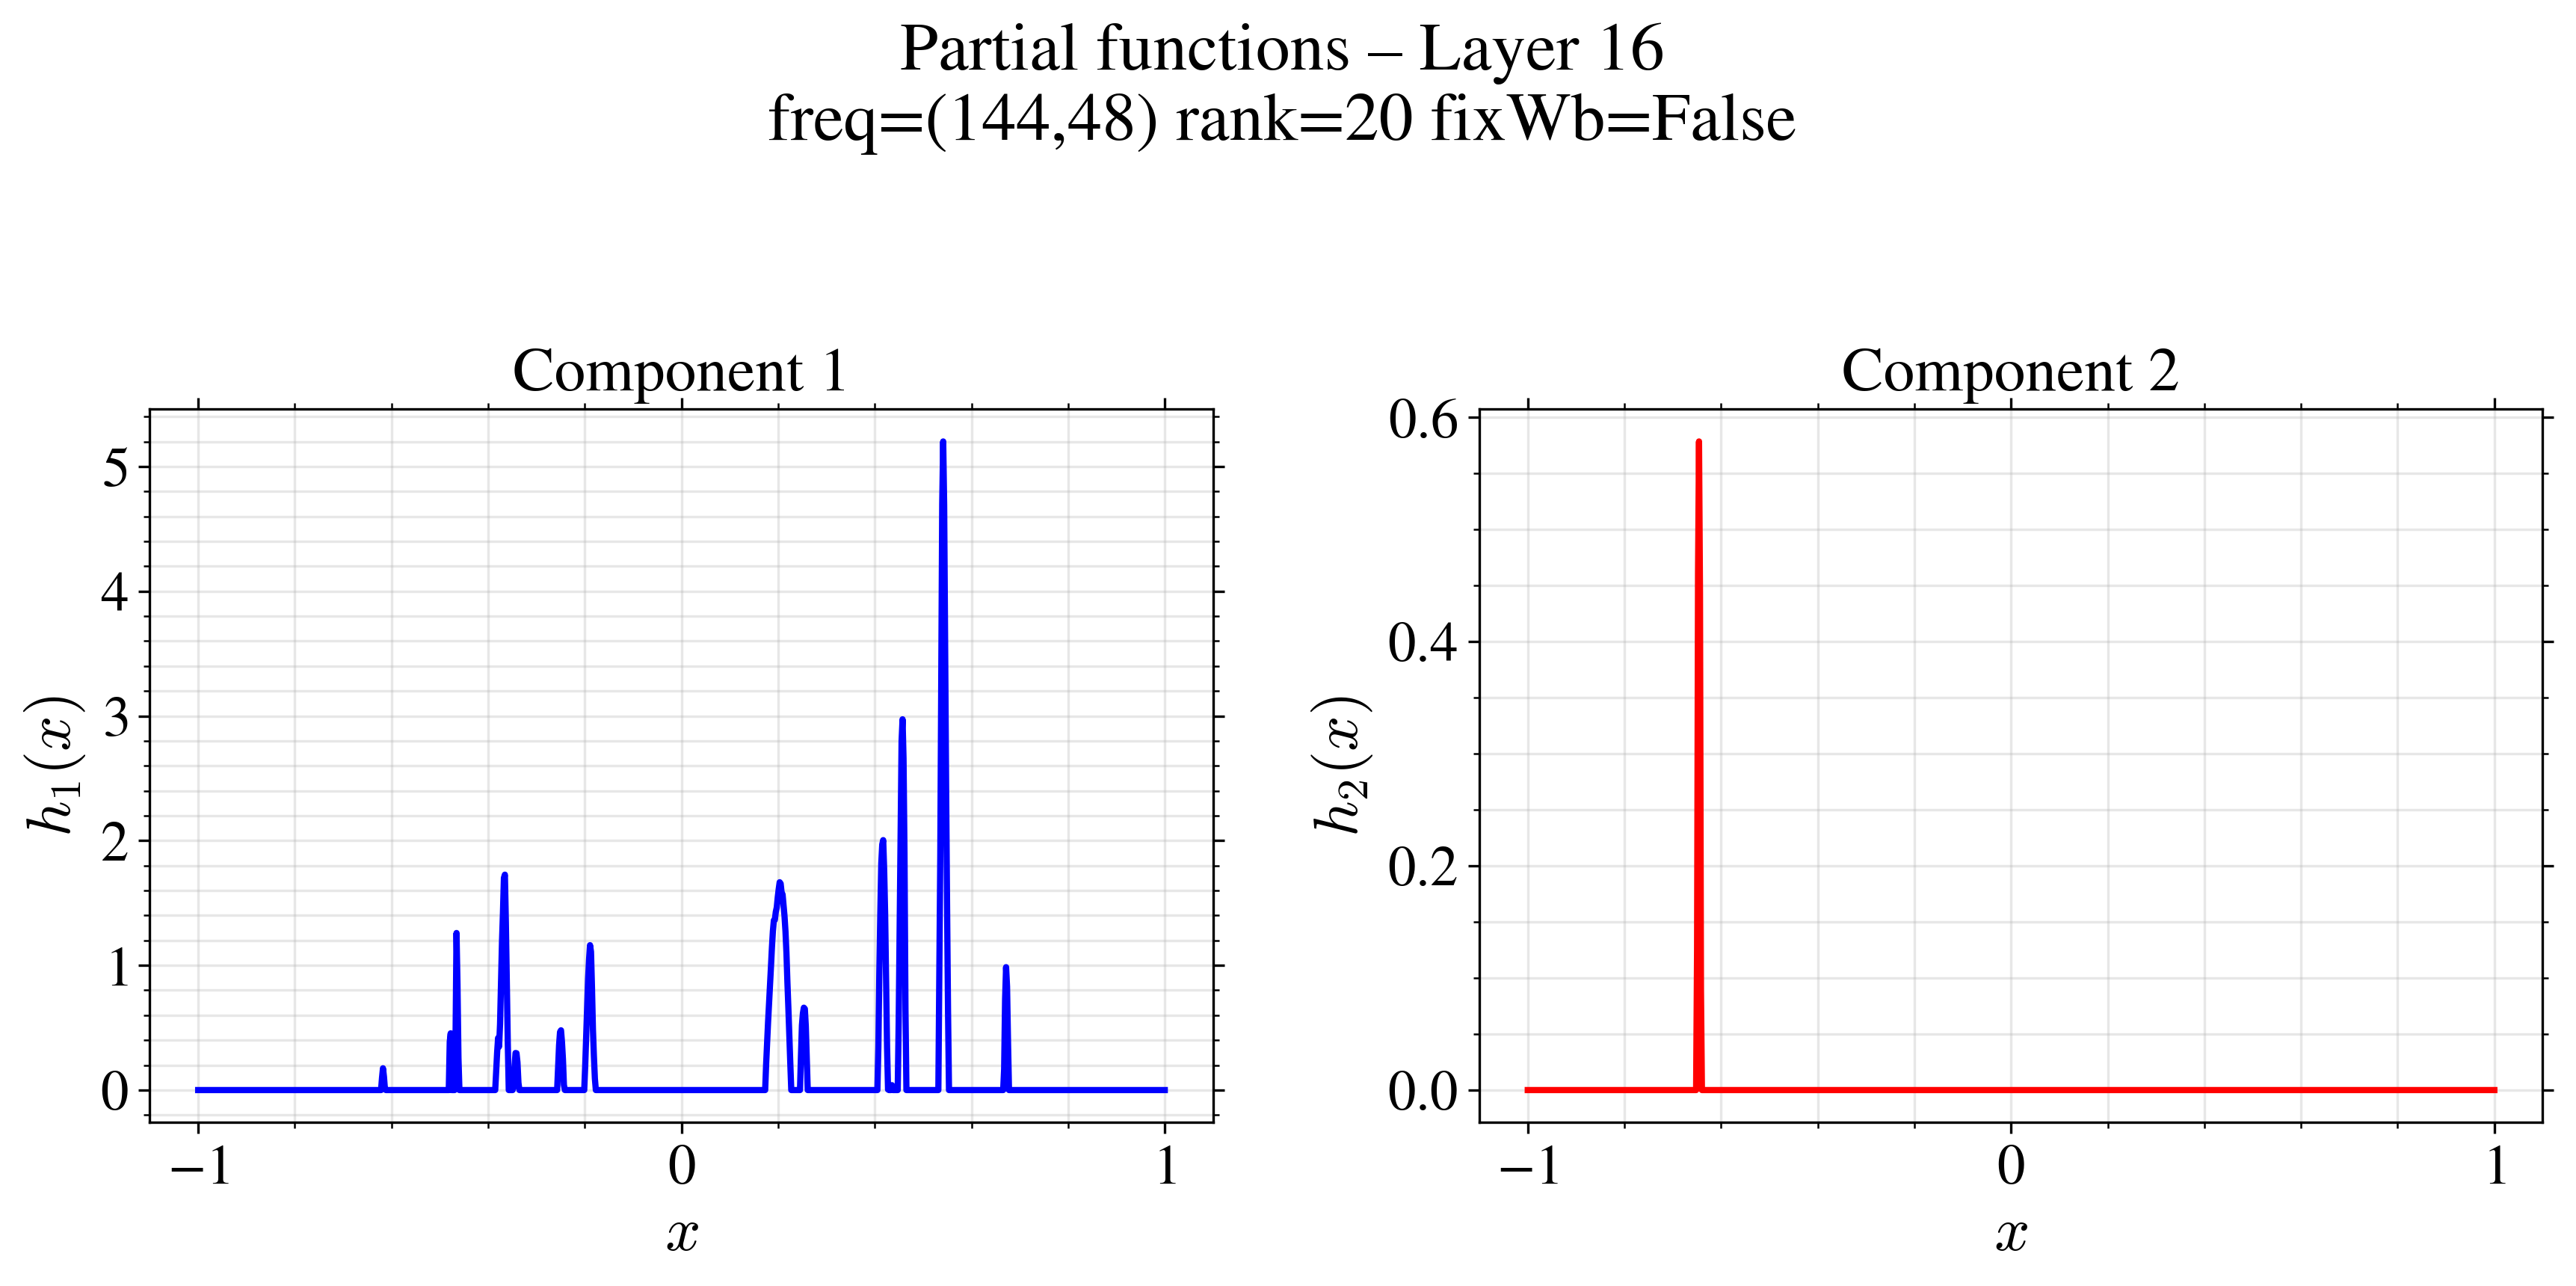
\includegraphics[width=0.47\textwidth]{results/paper_assets/paper_mlp_asymmetry_layer16.png}
\caption{RF-LR partial functions on the even high-frequency target and no-RF MLP asymmetry controls. The two layer-16 panels are enlarged to show that RF-LR keeps mirror structure at depth, while the no-RF MLP control remains visibly asymmetric.}
\label{fig:lowloss}
\end{figure*}

\paragraph{Counterexamples are useful.}
The completed checkpoint set separates into 12 partial-symmetric, 28 output-only/asymmetric, 92 intermediate, and 9 underfit runs.
For example, one rank-5 depth-3 $f_2$ run reaches test MSE $9.53\cdot10^{-4}$ with partial defect $2.62\cdot10^{-5}$.
In contrast, a rank-10 depth-1 $f_1$ run reaches test MSE $1.17\cdot10^{-4}$ but partial defect $2.17$.
Thus low output loss does not force internal symmetry; the positive low-rank regime is a real representation phenomenon.

\begin{figure}[!t]
\centering
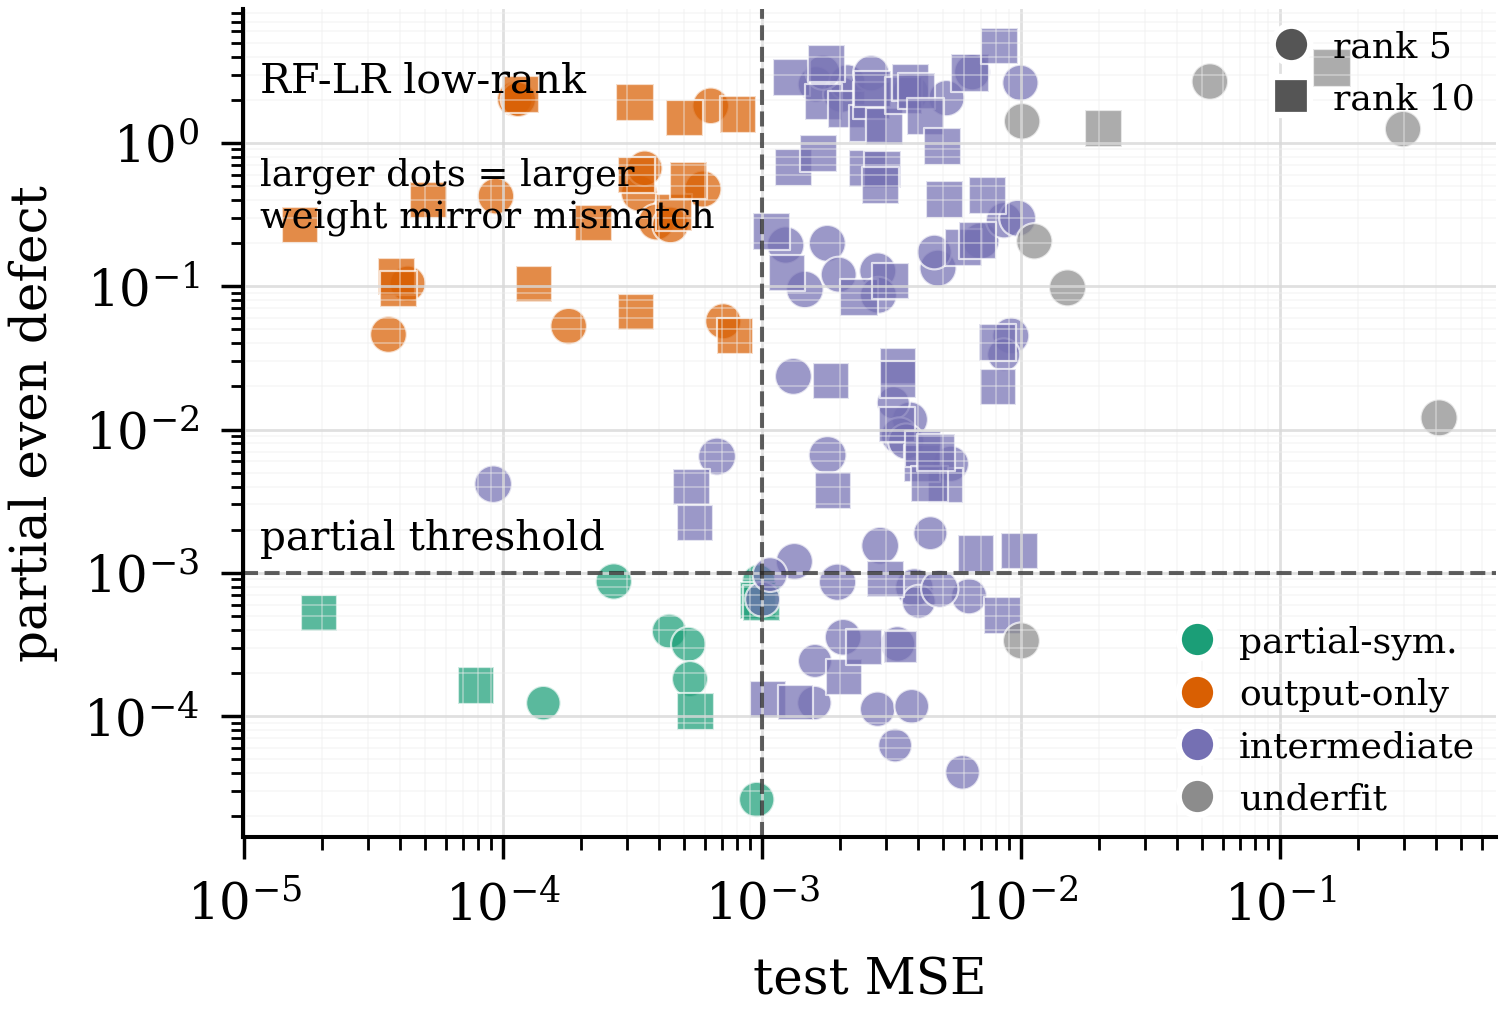
\includegraphics[width=0.98\linewidth]{results/paper_assets/paper_weightspace_regimes.png}
\caption{Weight-space symmetry diagnostic for completed one-dimensional RF-LR low-rank checkpoints. The axes are test MSE and active partial even defect; colors show functional regimes, circles/squares are rank $5/10$, and marker size is the median outgoing-weight mismatch between nearest mirror atoms $(a,b)$ and $(-a,b)$. Thus the plot should be read as a joint function/weight-space map: lower-left points are low-loss, internally symmetric, and have smaller mirror mismatch, while output-only points show that fitting the target does not force symmetric partials or organized mirror weights.}
\label{fig:mismatch}
\end{figure}

\paragraph{Batch-one multidimensional stress test.}
We then stress-test the strongest claim in two and three dimensions: symmetry can emerge from a fully asymmetric stochastic stream.
All runs below use batch size one, non-paired uniform training samples, Adam, width $512$, and low-rank bottlenecks with rank $8$ or $16$.
The training algorithm is deliberately simple: sample all random-feature matrices $A^{(\ell)}$ and biases $b^{(\ell)}$ once, freeze them, initialize only the channel mixers $B^{(\ell)}$, then run gradient descent on MSE through the full RF-LR forward map while updating only $B^{(\ell)}$.
For the multidimensional runs each optimizer step sees one unpaired point $x$, never the pair $(x,-x)$; best checkpoints are selected by held-out MSE, and all output, partial, and mirror-symmetry defects are computed only after training on a separate symmetric evaluation grid.
The 2D Gaussian run with rank $8$ and depth $3$ reaches test MSE $1.20\cdot10^{-5}$, output defect $6.91\cdot10^{-5}$ under $x\mapsto -x$, and active last-partial defect $6.62\cdot10^{-4}$.
The 3D quadratic run with rank $8$ and depth $3$ reaches test MSE $1.92\cdot10^{-4}$, output defect $9.76\cdot10^{-4}$, and active last-partial defect $1.81\cdot10^{-3}$.
Thus the phenomenon survives beyond the original one-dimensional setting while using rank-to-width ratio $8/512=1.56\%$.

\begin{figure}[!ht]
\centering
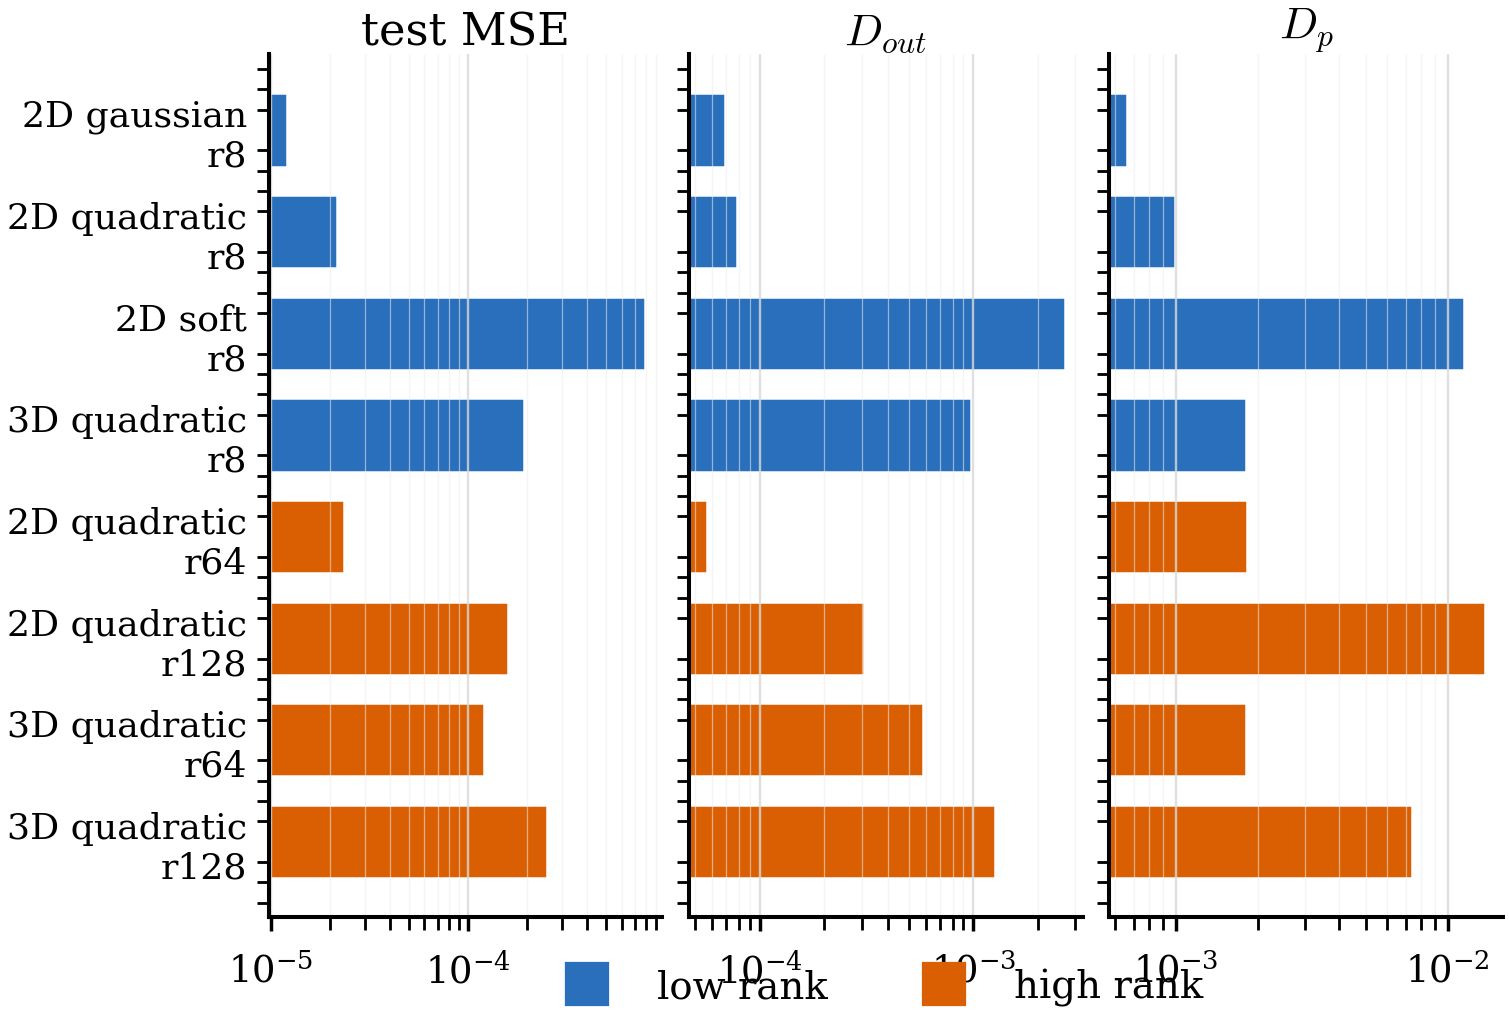
\includegraphics[width=0.83\linewidth]{results/paper_assets/paper_representative_bars.png}
\caption{Representative multidimensional RF-LR results as bars instead of a table. Blue bars are low-rank runs; orange bars are high-rank controls. Lower is better for all three metrics.}
\label{fig:main-results-bars}
\end{figure}

\begin{figure}[!ht]
\centering
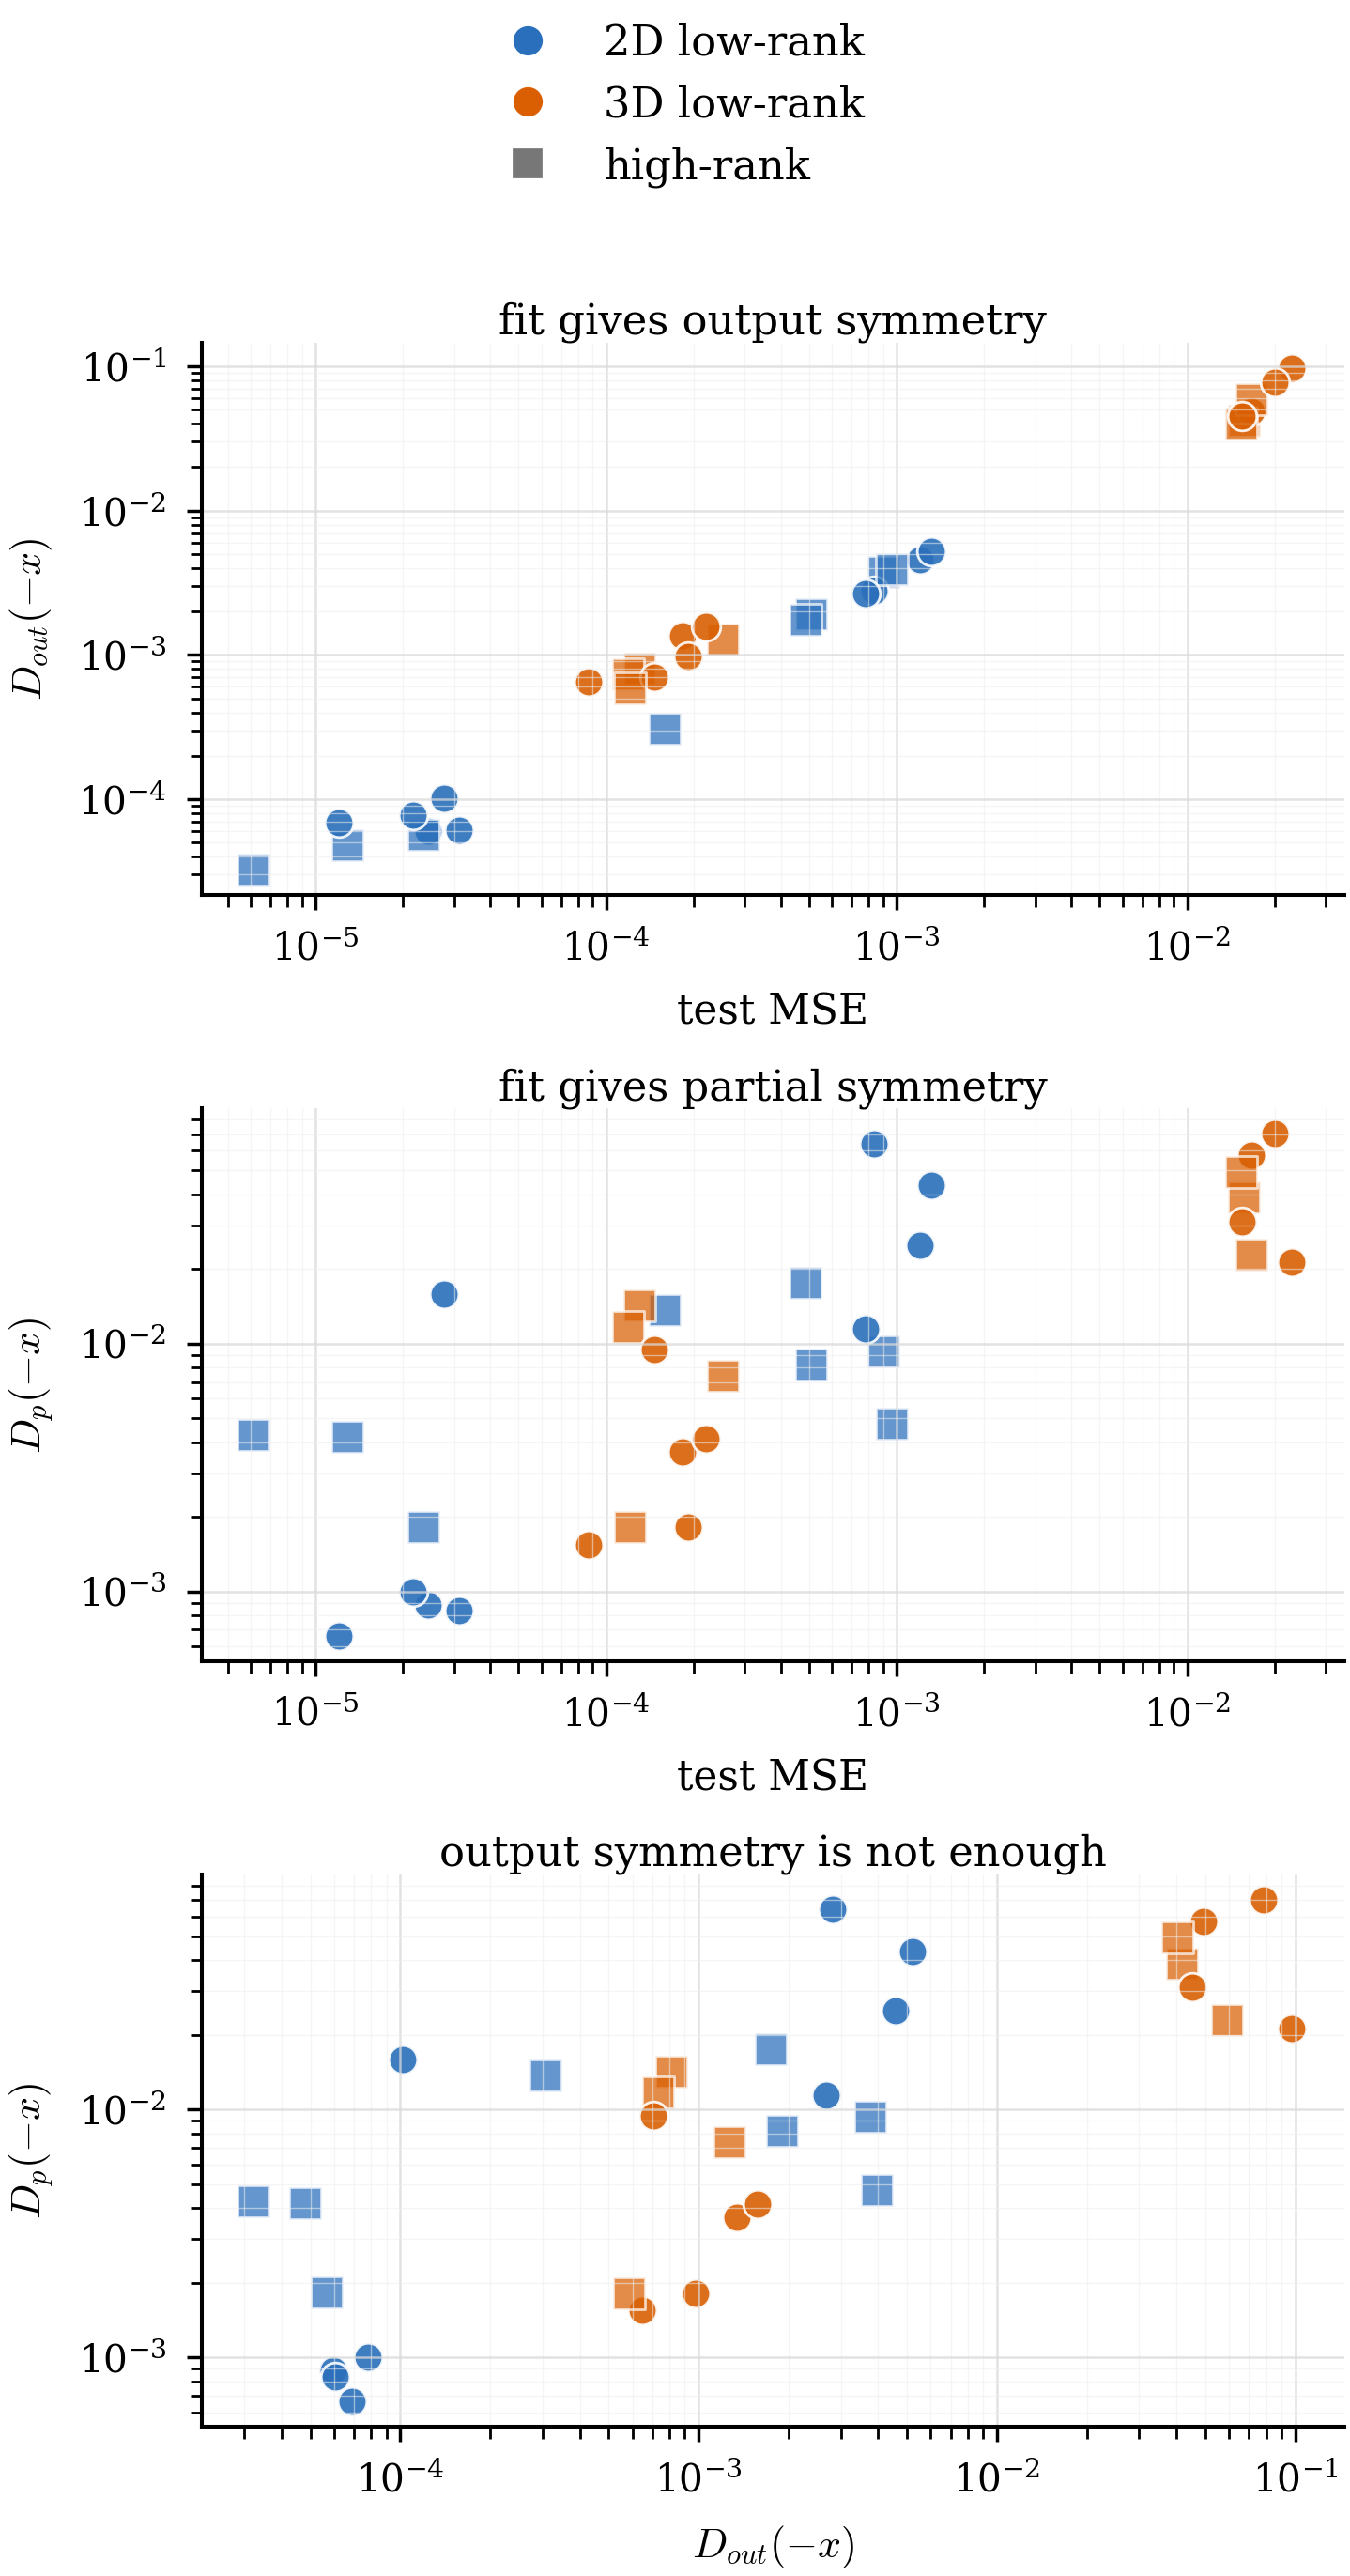
\includegraphics[width=0.83\linewidth]{results/paper_assets/paper_multidim_dashboard.png}
\caption{Multidimensional batch-one diagnostic. Circles are low-rank RF-LR, squares are higher-rank RF-LR. The three panels compare test error, output symmetry, and active-partial symmetry.}
\label{fig:multidim}
\end{figure}

Figure~\ref{fig:mismatch} is the main weight-space evidence.
It does not plot weights directly; instead it compresses the first-layer mirror-pair test into point size, so a good run should sit in the lower-left and avoid large markers.
This is precisely the regime where RF-LR has low loss, symmetric partials, and comparatively matched outgoing weights on mirror atoms.
Figure~\ref{fig:multidim} is the main multidimensional empirical summary: the important region is the lower-left corner, where both prediction error and symmetry defect are small.
Its conclusion is that batch-one asymmetric training can recover symmetric outputs and, in the best low-rank RF-LR cases, symmetric internal partial functions.
Figure~\ref{fig:main-results-bars} adds the rank ablation through low-rank and high-rank bars: more rank is not automatically better for internal symmetry, so the effect is not merely explained by capacity.

The key message for weight-space symmetries is that useful symmetries need not be imposed as exact architectural equivariances or explicit path-norm constraints \citep{neyshabur2015path}.
In low-rank random-feature networks, the optimizer can discover approximate, data-dependent symmetry in the trained low-rank weights.
This suggests a practical analysis program: compare models not only by their functions, but by whether the symmetry appears in their internal partials and mirror-organized parameters.

\section{Conclusion and Limitations}

Our final conclusion is that low-rank RF-LR networks recover functional symmetry better in the regimes where the target is actually learned, and that this recovery leaves a measurable trace in weight space.
The strongest evidence is not just small output defect: successful low-rank runs also show small active partial-function defects, meaning the symmetry is present inside the learned representation.
The rank ablation shows that simply increasing rank does not monotonically improve this internal symmetry, and the mirror-pair measurements show the corresponding parameter signature: nearest mirrored atoms have more compatible outgoing low-rank weights in the successful regime.
Thus the low-rank bottleneck acts as an implicit symmetry-recovery bias rather than merely as a parameter-count reduction.
The limitation is that the mirror metric is nearest-neighbor based and only probes the first layer; it supports the weight-space interpretation but remains weaker than the partial-function evidence.
Some harder 3D soft-axis targets still generalize poorly despite tiny training error, so the multidimensional claim is for the low-loss Gaussian and quadratic regimes, not all symmetric targets.

\bibliography{refs}
\bibliographystyle{icml2026}

\end{document}
